In this chapter we review the attributes of Rust that make it amenable for scientific computing, contrasting the experience of building and writing software with traditionally preferred compiled languages, specifically C, C++ and Fortran which are preferred implementation languages in scientific computing.

As we observed in chapter \ref{chpt:4:pyexafmm}, interpreted languages, despite their portability, great usability benefits and large ecosystems of numerical libraries, are constrained when used to implement high-performance scientific codes. For problems in which this overhead is untenable, compiled languages, such as C, C++ and Fortran are preferred. These languages require greater software engineering expertise, as developers are responsible for allocating memory, installing third party libraries, as well as building their software to target different hardware. These languages in a sense allow a developer to `do anything', of course only if one knows how to do it. The higher software engineering barrier manifests in a dizzying array of compilers, build systems, package managers, testing and documentation libraries and code organisation techniques. The notable thing about all of these optional choices is that it is relatively unclear which is the \textit{preferred} way of doing things, with novice developers likely to find a development strategy that `simply works' and stick to it. 

Rust stands in contrast to these traditionally preferred compiled languages for high performance scientific computing. Although it is comparably fast, it is relatively \textit{inflexible}. With a strongly preferred way of organising, testing, documenting and deploying software. This leads to significantly more uniform Rust code across projects and a steep, though relatively shorter, learning curve. This uniformity makes Rust code easier to share and port across different operating systems and hardware targets.

\subsection*{Package Managers and Build Systems}

For simple programs, it's tempting to use a compiler directly to create an executable, as in listing (\ref{code:ch_5:simple_compilation}). However, as a project's codebase expands with files defined in multiple directories and calls to external libraries often written in other programming languages, this simple one line appeal to a compiler will no longer be sufficient. One could always download their requisite software and install globally over the machine using a system package manager, and attempt to recompile. However, this quickly becomes untenable if one is developing for a range of hardware and operating system targets, or one needs to use different versions of external binaries and libraries. Therefore, software is usually constructed using a `build system'. This is catch all term that refers to a program that takes source files as input and produces a deployable set of binaries or libraries as an output. Classically, build systems were based on `Make' and `Autotools', these softwares generate `Makefiles' - which are recipes for constructing a piece of software given a set of source files and external dependencies. These are robust tools, but the onus is squarely with a developer for ensuring that all dependent libraries are visible to Make, and that the external packages are all of compatible versions.

To manage this complexity, builds are often defined using a metabuild system, most commonly CMake. CMake is a scripting language, and as a meta build system it takes a specification of local and third party dependencies and hardware targets, and generates Makefiles. CMake gives developers a great deal of flexibility, it is multi-platform, and language agnostic, however using it directly is not straightforward. Indeed, there is a significant body of literature discussing best practices with CMake \cite{scott2018professional}. However, CMake is not responsible for downloading and installing third party packages or verifying their relative compatibility, implementing its best practices is again left to users.

Approaches for reliable builds vary amongst projects, ranging from `low tech' readme driven solutions, in which a user follows a recipe of instructions, to more modern automated solutions. Figure (\ref{fig:ch_5:builds}) provides an overview of the different approaches taken. The lack of a uniform standard means that some projects go as far as to implement a custom build system, such as the Boost library \cite{boostbuild2022github}.

Keeping on top of packages, which are constantly being iterated upon independently, and may support different features with each release, is nearly impossible to do manually. Furthermore, one may want to support a specific set of packages, and respectively versions, for a given hardware or operating system target, but a different set for a different build of the same software. This has led to the development of `package managers' which are a catch all term for softwares that can download and install required software for you, and often verify whether version constraints are satisfied too. Package managers can be delineated into `system package managers', which download operating system specific packages written in any language globally on your machine, and `language specific package managers' which focus only on packages written in a given target language, but are operating system agnostic from a user's perspective.

In terms of system package managers Linux examples include apt, yum and debian, for MacOS there is Homebrew, and Chocolatey for Windows. These can handle both source installations, in which source code is compiled upon download, as well as binary installation, in which pre-built binaries matching your hardware constraints are installed. Binary installation is often preferred, as it is faster, and often reflects a stable software release. Language specific package managers, such as pip for Python, can handle dependencies written in these languages only. Developing your own packages for system package managers is not developer friendly, official package repositories of Linux package managers are moderated by their respective maintainers, though it is possible to set up a personal repository this is quite a sophisticated approach for simple research outputs. The simple alternative, pursued by up to 26 \% of surveyed C++ softwares (see fig. (\ref{fig:ch_5:builds})), is to simply add third party software as a submodule. Often to ease installation, C++ libraries are shipped as `header only' libraries, this makes them easy to install, requiring only an \pythoninline{#include}. However by using such techniques a project can quickly grow to contain thousands, to millions of lines of code, much of it in dependencies. Compiling from source has the potential to be a painstakingly slow process, and must be repeated for every combination of hardware and operating system targets one wants to run on.

\begin{figure}
    \centerline{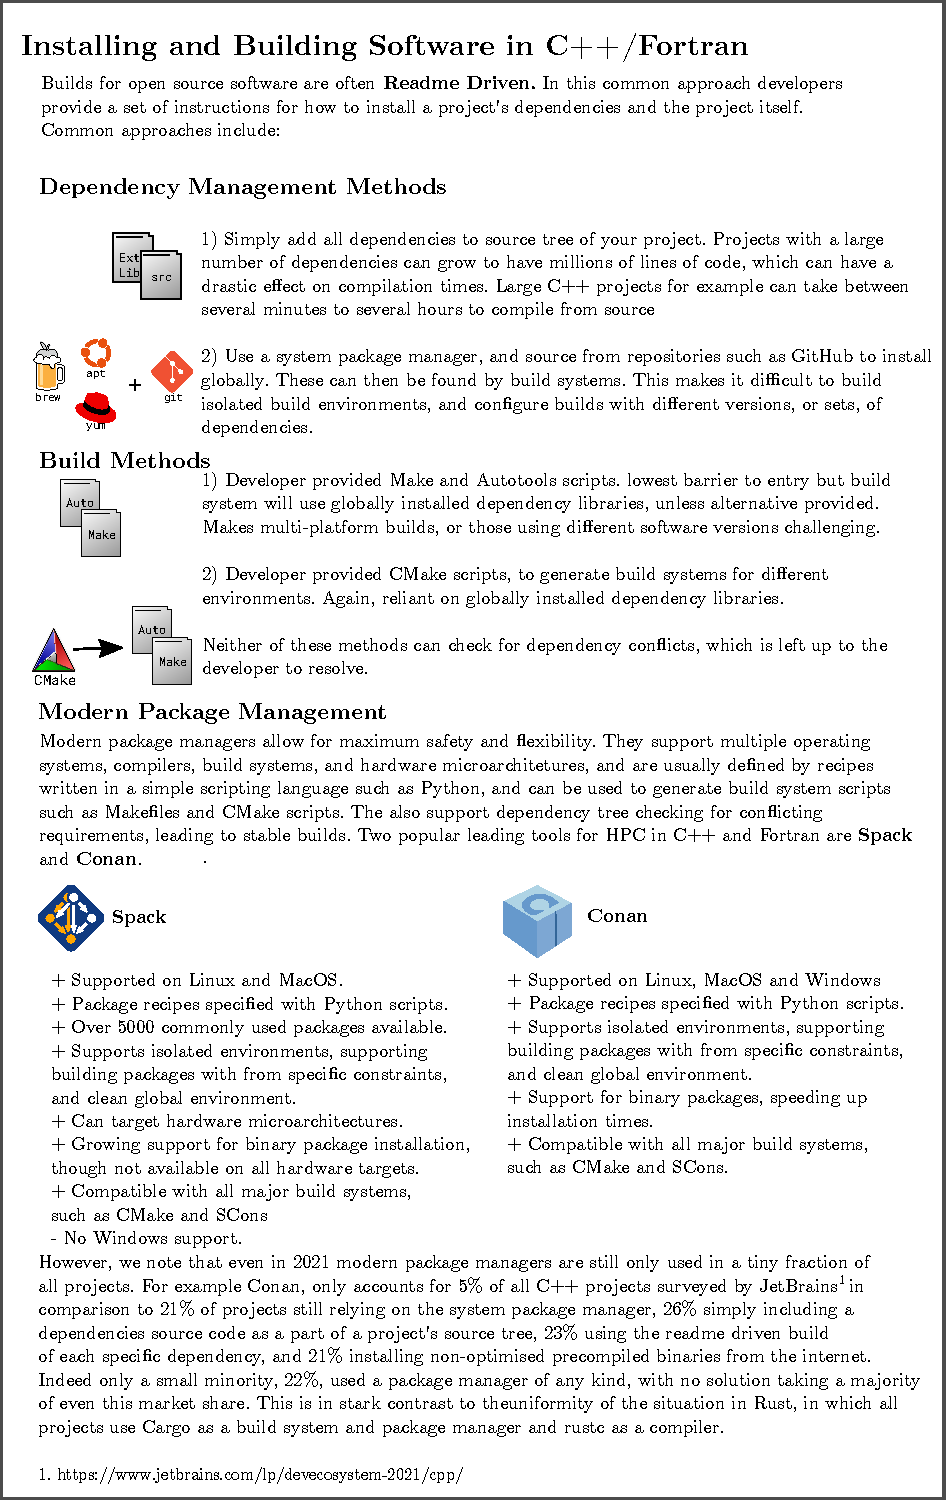
\includegraphics[width=0.95\linewidth]{ch_5/builds.pdf}}
    \caption{An overview of building software in other compiled languages.}
    \label{fig:ch_5:builds}
\end{figure}

With the exception of Fortran, which has made recent strides to develop a standardised modern package manager and build system, inspired by Rust's Cargo \cite{fpm2022github}, C and C++ do not have a single officially supported package manager or build system. The resulting landscape is a multitude of package managers \cite{spack2022github, vcpkg2022github, conan2022github} and build systems \cite{meson2022github, bazel2022github, scons2022github} a few of which we have cited here, all of which replicate each others functionality, none of which are universally accepted or implemented across projects nor officially supported by the C++ software foundation.

\bashexternal[basicstyle=\footnotesize, caption={Compiling a simple \texttt{source\_code.cpp} into a \texttt{compiled\_binary} file from a terminal.}\label{code:ch_5:simple_compilation}]{simple_compilation.sh}

Recent years have seen the bundling of package managers \textit{with} build systems, resulting in softwares that can simply take source files, and a set of dependencies, and resolve a single binary output for a given hardware and software target. Examples include Conda for Python, and Rust's Cargo system. These modern efforts are able to compile both source and binary packages for all operating systems, and can target a wide range of hardware architectures. Furthermore, the trend has been towards the specification of project dependencies in a single structured text file (see listing (\ref{code:ch_5:simple_cargo})), which is then handled by the package manager with no further user effort. Efforts have been in this direction for older compiled languages, the most notable examples being Spack and Conan (see fig. (\ref{fig:ch_5:builds})). Importantly, in the case of Rust, Cargo is officially supported and shipped as a core part of its runtime. In contrast to C, C++ and Fortran, Rust has a \textit{single} officially supported compiler, rustc. By taking global decisions for all software written in Rust, a significant burden is removed from developers of Rust software, similar to the situation in many interpreted languages. Indeed Cargo builds are often executed in a \textit{single line}, eradicating the complex readme driven builds common in other compiled languages. For the project specified by listing (\ref{code:ch_5:simple_cargo}) can be compiled from a terminal with the command: \texttt{cargo build}.

\bashexternal[basicstyle=\footnotesize, caption={An example of a simple \texttt{Cargo.toml} file for a Rust project, with source as well as binary dependencies.}\label{code:ch_5:simple_cargo}]{snippets/Cargo.toml}

\subsection*{Code Organisation and Quality}

Rust introduces many ergonomic features for code organization. The most novel features, which may not be familiar to those coming from other compiled languages, are the concepts of traits, lifetimes and the borrow checker.

\subsubsection*{Traits}

Traits are Rust's system for specifying shared behaviour and building abstraction, constituting a wholesale replacement of object oriented programming, with its inheritance based hierarchies. Traits only enforce \textit{behaviour}, and therefore are strictly less brittle than object orientation which enforces a type. We provide some example syntax in listing (\ref{code:ch_5:simple_traits}), and contrast it to equivalent object oriented code in ;listing (\ref{code:ch_5:simple_class}). We notice that the object oriented code has a built in hierarchy, which means that adding shared behaviour will effect our \pythoninline{MyType} type, and everything that subsequently depends on it, in contrast to the trait based code in which we can inject new behaviour into \pythoninline{MyType}, its subsequent dependents we only need to know about the traits and their associated interfaces that they themselves rely on. This means that one can focus solely on the behaviour implicit in a given Trait, rather than having to comb through a potentially complex hierarchy of objects and inheritance to understand what a given line of code is doing, making large Rust projects significantly more readable than their object oriented equivalents.

Traits can be seen to specify shared behaviour in a bottom up manner, as opposed to top down object orientation, new features can be injected into existing types. This is useful for scientific programming, as we are usually concerned with data oriented programming. As we saw in chapter \ref{chpt:4:pyexafmm} exploring data oriented programming in Python, object oriented design obfuscates operations on the data itself behind abstraction.

\rustexternal[basicstyle=\footnotesize, caption={An example of a trait implemented on a custom type.}\label{code:ch_5:simple_traits}]{snippets/trait.rs}

\pythonexternal[basicstyle=\footnotesize, caption={An example of behaviour in listing (\ref{code:ch_5:simple_traits}) implemented in an object oriented manner}\label{code:ch_5:simple_class}]{snippets/pyclass.py}

This isn't to say similar syntax isn't available in other compiled languages. In C++20, `concepts' were introduced as a trait like mechanism to specify interfaces. However, as with many things in C++, this isn't enforced and it is up to a user to choose to implement their code in this manner. This is borne out in the fact that concepts are \textit{nominally typed}, and therefore don't enforce behaviour as in Rust's \textit{structurally typed} traits. The implication of this being that a type may `accidentally' implement a concept, if it happens to define its relevant methods. A consequence of this is that a valid C++ program can contain a confusing mix of trait based, and object oriented code, with a a reader then dependent on documentation to understand a software's behaviour, and what has been enforced and where, by the developer.

\subsubsection*{Lifetimes and the Borrow Checker}

Another new Rust concept for developers coming from other compiled languages is the idea of `lifetimes' and `ownership'. Every reference in Rust has an associated lifetime, and a singular `owner'. Which enforce the programming pattern of `resource allocation is initialisation' (RAII) as a feature of the Rust compiler. The basic rule is that references are owned within a scope, and dropped when out of scope. We provide a basic example in listing (\ref{code:ch_5:borrowing}), in a Rust context RAII is better encapsulated by another acronym `destructors run at exit scope' (DRES). 

\rustexternal[basicstyle=\footnotesize, caption={A demonstration of basic rules of borrowing and ownership.}\label{code:ch_5:borrowing}]{snippets/ownership.rs}

Lifetimes are a Rust concept that guarantees that any references to a resource live at least as long as the resource itself. The main aim of this to prevent dangling references, whereby references to unintended data, or de-allocated data, are not present in the compiled binary. This removes a large class of common bugs from Rust software such as dangling pointers, and double free errors. We illustrate this in listing (\ref{code:ch_5:lifetimes}), which won't compile as the inner scope defines a value \pythoninline{x}, which doesn't survive into the outer scope. 

\rustexternal[basicstyle=\footnotesize, caption={A demonstration of lifetimes as a function of scope. This example is adapted from the Cargo book \cite{klabnik2019rust}.}\label{code:ch_5:lifetimes}]{snippets/lifetimes.rs}

Rust's compiler enforces ownership and lifetime rules uses a program called the `borrow checker' to ensure that all references, and lifetimes, are referring to valid memory locations at \textit{compile time} without the need for a runtime garbage collector. This is a huge advantage over other compiled languages, for example memory related bugs have been found to constitute as much as 70 \% of all security bugs at Microsoft \cite{microsoft2019}. From a scientific programming perspective, handling memory additionally bogs down algorithm development, iteration, and ultimately publication, and was one of the major contributing factors in the push towards interpreted languages in recent decades. Again, this is not to say similar features do not exist in other compiled languages. C++ has its notion of `smart pointers', which enforce RAII principles too, however as with other features in C++, this is a library feature rather than a core part of its compiler, or language specification, making it optional and unenforced. 

The benefits of Rust's memory system extend to parallel code too. A wide variety of programming paradigms for parallel computation with threads exist, in scientific software we often use OpenMP, which uses the shared memory paradigm, such that all threads operate on the same data. In this setting one of the most common bugs is a data race condition, whereby multiple threads attempt to write to the same memory location. Rust's ownership system enforces the atomicity of all memory operations, by passing ownership between threads, as only a single mutable reference can exist to a piece of memory Rust is able to prevent data races at compile time. Although atomic operations are available in OpenMP, or other shared memory systems, the benefit of Rust is that we know that our compiled code \textit{cannot} contain this bug, without having to rely on unit tests for expected behaviour.

\subsubsection*{Code Quality}

Rust's runtime includes a test runner, a documentation generator, and a code formatter. As with other Rust features, these are maintained in lock step with the language specification, and with reference to other Rust developments. This imposes universal constraints on all Rust projects, allowing for objectively defined `good' Rust code, rather than relying on various standards of best practices that vary between projects and organisations.

\subsection*{Rust's Scientific Ecosystem and Foreign Libraries}

Despite being a young language, Rust already supports a mature ecosystem of libraries for scientific computing with high-level multithreading support \cite{rayon2018github}, numerical data containers \cite{ndarray2022github}, and tools for generating interfaces to Python via its C ABI \cite{maturin2022github}.

Many tools are yet to be ported into native Rust, however high quality bindings exist for core tools such as MPI \cite{rsmpi2018github}, BLAS and LAPACK \cite{blaslapackrust2022github}, which are relatively easy to interface into Rust via its C ABI. The problem with interfacing with tools written in other languages is again related to building software, however Cargo offers tools to build software written in other languages and integrate it with Rust code via the \pythoninline{build} crate, which allows one to leverage existing build systems written for software written in foreign languages. This detracts from the benefits offered by Cargo as a unified package manager and build system, raising similar problems to those encountered when building software in other compiled languages. However, we observe that this remains a concern of the software's developer, who is responsible for providing build scripts for the operating systems and hardware platforms that they wish to support, and from a downstream user perspective their build process remains the same as with pure Rust packages, where the dependency is defined in their \pythoninline{Cargo.toml} file.

We also note that Rust is missing key tools for scientific computing, such as a code generation for GPUs, as well as for advanced optimised advanced linear algebra routines, especially for sparse matrices. However, both of these applications are an active area of development.

\subsection*{Conclusion}

Rust's syntax and program structure are strongly opinionated, its build system emphasises simplicity and portability, and its ecosystem for scientific computing is rapidly developing. A small software team, as is common in academic settings, writing in Rust are effectively able to maintain and deploy Rust projects to a wide variety of platforms, from laptops to supercomputers. Rust's simplified build process results in minimal configuration for users, encouraging the widespread adoption of Rust projects.
